\documentclass[tikz]{standalone}
\usetikzlibrary{arrows,shapes.geometric,positioning,matrix}
\tikzset{
  ishikawa/.style={align=center, inner sep=0pt},
  matter/.style  ={rectangle, minimum size=6mm, very thick, draw=red!70!black!40,
    top color=white, bottom color=red!50!black!20, font=\itshape},
  level_1/.style ={ellipse, node distance=60pt, minimum size=6mm, very thick,
    draw=red!50!black!50, top color=white, bottom color=red!50!black!20, font=\itshape},
  level_2/.style={rectangle, minimum size=6mm, font=\itshape, font=\tiny}}
\tikzset{
  rows/.style 2 args={@/.style={row ##1/.style={#2}},@/.list={#1}},
  cols/.style 2 args={@/.style={column ##1/.style={#2}},@/.list={#1}},
}
\begin{document}
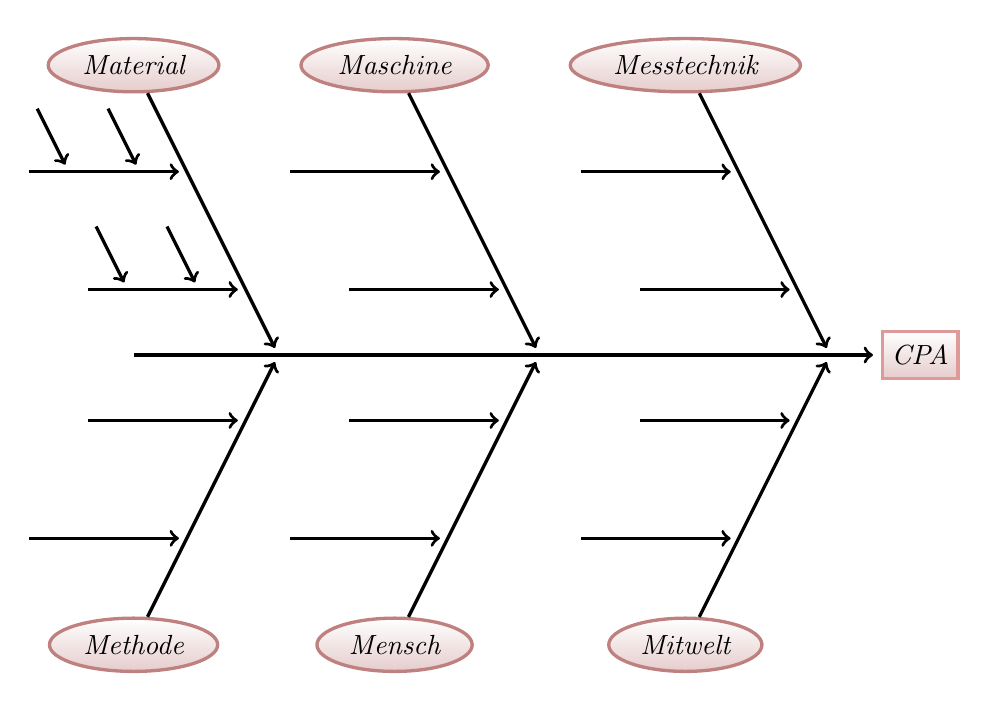
\begin{tikzpicture}
\matrix[
  matrix of nodes,
  row sep=3cm,
  column sep=1cm,
  rows={1,3}{nodes=level_1},
  rows=2{nodes=matter,anchor=center}
] (m) {
Material & Maschine & Messtechnik & \\
         &          &             & CPA \\
Methode  & Mensch   & Mitwelt     & \\
};
\path[very thick,
  to arr/.style={->, shorten <=+0pt, shorten >=+.1cm},
  fr arr/.style={<-, shorten >=+0pt, shorten <=+.1cm}]
  [to arr]
  (m-1-1|-m-2-4) edge (m-2-4)
  \foreach \r [evaluate={\xslant=\r==3?.5:-.5;}] in {1,3}{
    \foreach \c in {1,...,3}{
      (m-\r-\c) edge[xslant=\xslant]
        coordinate[pos=.3]   (@-\r-\c-1)
        coordinate[near end] (@-\r-\c-2) (m-\r-\c|-m-2-4)
      [fr arr]
      (@-\r-\c-1) edge ++ (left:2cm)
      (@-\r-\c-2) edge ++ (left:2cm)
    }
  }
  \foreach \prt in {1,2}{
  (@-1-1-\prt) --
    coordinate[pos=.3]   (@1-\prt)
    coordinate[near end] (@2-\prt) ++ (left:2cm)
  [fr arr]
  (@1-\prt) edge ++ ([xslant=-.5]up:.8cm)
  (@2-\prt) edge ++ ([xslant=-.5]up:.8cm)
  };
\end{tikzpicture}
\end{document}
